\begin{center}
\Huge
Tangentligninger og hældningsfelter
\end{center}


\section*{Tangentlinjer}
\stepcounter{section}

Hvis vi har en differentialligning, så ved vi, at den både har en generel løsning, der består af dens uendeligt mange partikulære løsninger. Til hvert punkt er det oftest let at finde hældningen af tangenten til den partikulære løsning, der går gennem netop dette punkt. Den differentierede optræder jo ofte eksplicit i differentialligningen. 

Vi vil gennem eksempler se, hvordan vi bestemmer tangentligninger til integralkurver. 

\begin{exa}
	Vi betragter differentialligningen 
	\begin{align*}
		y' = xy. 
	\end{align*}
	Vi ved, at der findes en løsning gennem punktet $(3,2)$, og vi vil gerne bestemme ligningen for tangenten til løsningskurven gennem dette punkt. Vi udnytter, at
	en ret linje kan skrives som 
	\begin{align*}
		y = ax+b,
	\end{align*}
	og vi ved, at hældningen er givet ved $y'(x)$ i punktet $(3,2)$. Hældningen er derfor
	\begin{align*}
		a = y'(3) = 3\cdot 2 = 6.
	\end{align*}
	Vi ved også, at linjen går gennem $(3,2)$. Derfor må der gælde, at 
	\begin{align*}
		2 = 6\cdot 3 + b \ \Leftrightarrow \  b =-16. 
	\end{align*}
	Ligningen for tangenten til løsningskurven gennem $(3,2)$ er derfor
	\begin{align*}
		y = 6x-16.
	\end{align*}
\end{exa}


\section*{Hældningsfelter}
\stepcounter{section}
Et hældningsfelt er en måde at visualisere løsningskurverne til en differentialligning. Hældningsfelterne består af små stykker af tangentlinjer indtegnet i et koordinatsystem. 
\begin{exa}
	Vi betragter differentialligningen
	\begin{align*}
		y' = xy.
	\end{align*}
	Et hældningsfelt for denne differentialligning kan ses på Fig. \ref{fig:hel1}.
	\begin{figure}[H]
		\centering
		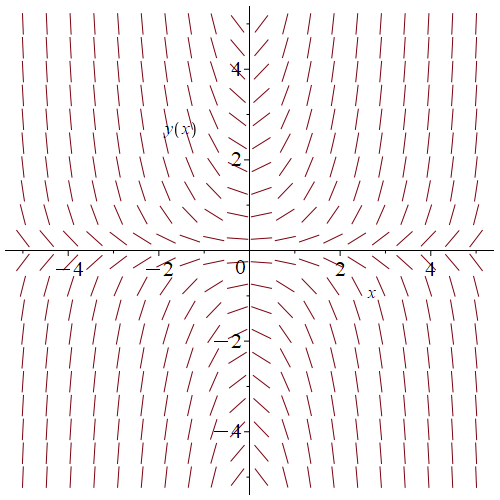
\includegraphics[width=0.6\textwidth]{Billeder/xyhf.png}
		\caption{Hældningsfelt for $y' = xy$.}
		\label{fig:hel1}.
	\end{figure}
\end{exa}

\begin{exa}
	Vi betragter differentialligningen 
	\begin{align*}
		f'(x) = f(x)+x.
	\end{align*}
	Et hældningsfelt for denne differentialligning kan ses på Fig. \ref{fig:hel2}.
	\begin{figure}[H]
		\centering
		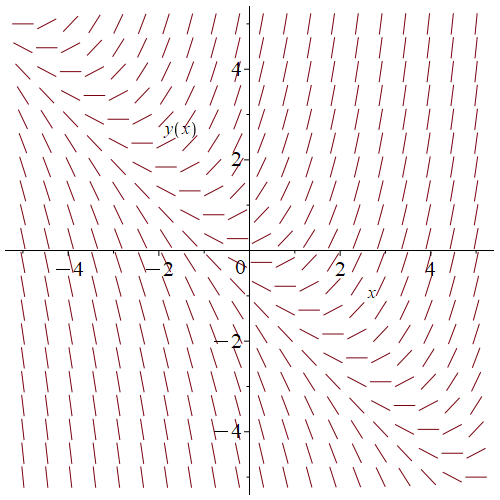
\includegraphics[width=0.6\textwidth]{Billeder/xpyhf.png}
		\caption{Hældningsfelt for $y' = x+y$.}
		\label{fig:hel2}.
	\end{figure}
\end{exa}

\section*{Opgave 1}
\begin{enumerate}[label=\roman*)]
	\item Bestem tangentligningen for integralkurven til differentialligningen
	\begin{align*}
		y' = x + y
	\end{align*}
	gennem punktet $(5,-6)$.
	\item Bestem tangentligningen for integralkurven til differentialligningen
	\begin{align*}
		\frac{\intd y}{\intd x} = \frac{y}{x}
	\end{align*}
	gennem punktet $(-2,3)$.
	\item Bestem tangentligningen for integralkurven til differentialligningen 
	\begin{align*}
		f'(x) = \frac{x}{y} 
	\end{align*}
	gennem punktet $(18,6)$.
\end{enumerate}

\section*{Opgave 2}
\begin{enumerate}[label=\roman*)]
	\item Et hældningsfelt for differentialligningen
	\begin{align*}
		y' = \frac{y}{x}
	\end{align*}
	er givet ved
	\begin{center}
		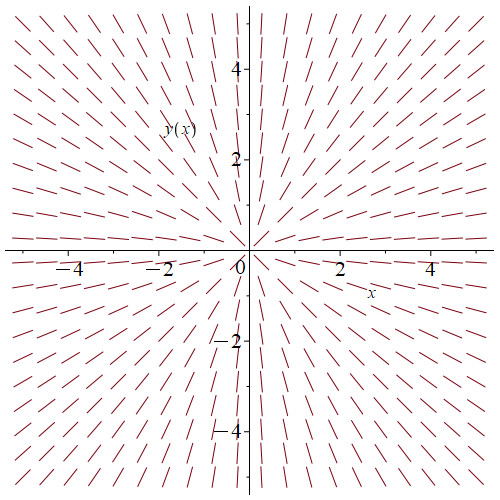
\includegraphics[width = 0.5\textwidth]{Billeder/O1.png}
	\end{center}
	Tegn to partikulære løsning gennem punkterne $(0,0)$ og $(0,2)$.
	\item Et hældningsfelt for differentialligningen
	\begin{align*}
		y' = x + y
	\end{align*}
	er givet ved
	\begin{center}
		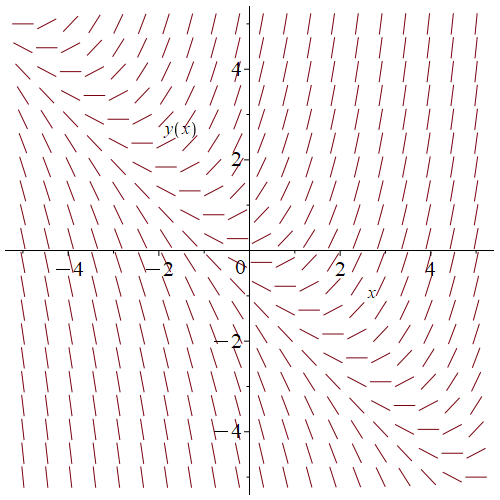
\includegraphics[width = 0.5\textwidth]{Billeder/O2.png}
	\end{center}
	Tegn to partikulære løsning gennem punkterne $(0,2)$ og $(-2,0)$.
	\item Et hældningsfelt for differentialligningen
	\begin{align*}
		f'(x) = 2x
	\end{align*}
	er givet ved
	\begin{center}
		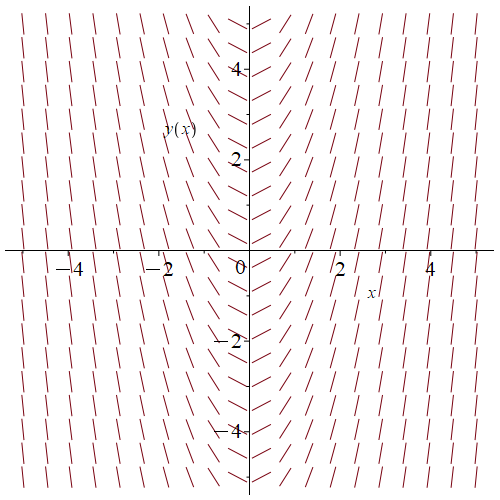
\includegraphics[width = 0.5\textwidth]{Billeder/O3.png}
	\end{center}
	Tegn to partikulære løsning gennem punkterne $(0,-2)$ og $(0,2)$.
	\item Et hældningsfelt for differentialligningen
	\begin{align*}
		y' = \frac{x}{y}
	\end{align*}
	er givet ved
	\begin{center}
		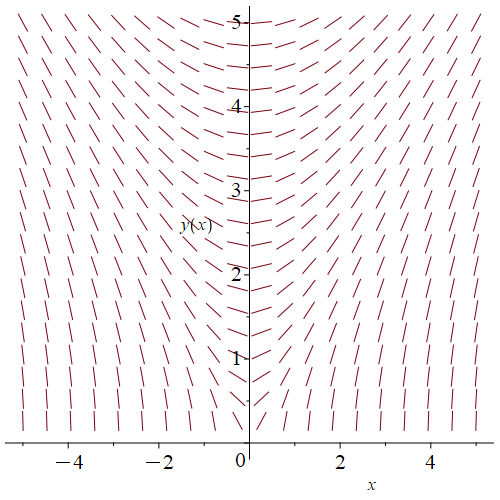
\includegraphics[width = 0.5\textwidth]{Billeder/O4.png}
	\end{center}
	Tegn to partikulære løsning gennem punkterne $(0,1)$ og $(0,4)$.
\end{enumerate}

\section*{Opgave 3}

\begin{enumerate}[label=\roman*)]
	\item Bestem tangentligningen for løsningskurven til differentialligningen
	\begin{align*}
		y' = 5y
	\end{align*}
	i punktet (2,4).
	\item Det oplyses, at den generelle løsning til differentialligningen er givet ved
	\begin{align*}
		y(x) = ce^{5x}.
	\end{align*}
	Vis, at dette er en løsning.
	\item Bestem den partielle løsning, der går gennem punktet (2,4).
	\item Bestem nu tangentligningen for denne funktion i punktet (2,4), og sammenlign dit 
	resultat med i).
\end{enumerate}

\section*{Opgave 4}
\begin{enumerate}[label=\roman*)]
	\item Bestem tangentligningen for løsningskurven til differentialligningen
	\begin{align*}
		\frac{\intd y}{\intd x} = \frac{x}{y}
	\end{align*}
	i punktet (6,3).
	\item Det oplyses, at den generelle løsning til differentialligningen er givet ved
	\begin{align*}
		y(x) = \frac{1}{x^2+k}.
	\end{align*}
	Vis, at dette er en løsning.
	\item Bestem den partielle løsning, der går gennem punktet $\left(3,\frac{1}{4}\right)$.
	\item Bestem nu tangentligningen for denne funktion i punktet $\left(3,\frac{1}{4}\right)$
	, og sammenlign dit 
	resultat med i).
\end{enumerate}
